%% abtex2-modelo-trabalho-academico.tex, v-1.9.7 laurocesar
%% Copyright 2012-2018 by abnTeX2 group at http://www.abntex.net.br/ 
%%
%% This work may be distributed and/or modified under the
%% conditions of the LaTeX Project Public License, either version 1.3
%% of this license or (at your option) any later version.
%% The latest version of this license is in
%%   http://www.latex-project.org/lppl.txt
%% and version 1.3 or later is part of all distributions of LaTeX
%% version 2005/12/01 or later.
%%
%% This work has the LPPL maintenance status `maintained'.
%% 
%% The Current Maintainer of this work is the abnTeX2 team, led
%% by Lauro César Araujo. Further information are available on 
%% http://www.abntex.net.br/
%%
%% This work consists of the files abntex2-modelo-trabalho-academico.tex,
%% abntex2-modelo-include-comandos and abntex2-modelo-references.bib
%%

% ------------------------------------------------------------------------
% ------------------------------------------------------------------------
% abnTeX2: Modelo de Trabalho Academico (tese de doutorado, dissertacao de
% mestrado e trabalhos monograficos em geral) em conformidade com 
% ABNT NBR 14724:2011: Informacao e documentacao - Trabalhos academicos -
% Apresentacao
% ------------------------------------------------------------------------
% ------------------------------------------------------------------------

\documentclass[
	% -- opções da classe memoir --
	12pt,				% tamanho da fonte
	openright,			% capítulos começam em pág ímpar (insere página vazia caso preciso)
	twoside,			% para impressão em recto e verso. Oposto a oneside
	a4paper,			% tamanho do papel. 
	% -- opções da classe abntex2 --
	%chapter=TITLE,		% títulos de capítulos convertidos em letras maiúsculas
	%section=TITLE,		% títulos de seções convertidos em letras maiúsculas
	%subsection=TITLE,	% títulos de subseções convertidos em letras maiúsculas
	%subsubsection=TITLE,% títulos de subsubseções convertidos em letras maiúsculas
	% -- opções do pacote babel --
	english,			% idioma adicional para hifenização
	french,				% idioma adicional para hifenização
	spanish,			% idioma adicional para hifenização
	brazil				% o último idioma é o principal do documento
	]{abntex2}

% ---
% Pacotes básicos 
% ---
\usepackage{lmodern}			% Usa a fonte Latin Modern			
\usepackage[T1]{fontenc}		% Selecao de codigos de fonte.
\usepackage[utf8]{inputenc}		% Codificacao do documento (conversão automática dos acentos)
\usepackage{indentfirst}		% Indenta o primeiro parágrafo de cada seção.
\usepackage{color}				% Controle das cores
\usepackage{graphicx}			% Inclusão de gráficos
\usepackage{microtype} 			% para melhorias de justificação
\usepackage{placeins}

% ---
		
% ---
% Pacotes adicionais, usados apenas no âmbito do Modelo Canônico do abnteX2
% ---
\usepackage{lipsum}				% para geração de dummy text
% ---

% ---
% Pacotes de citações
% ---
\usepackage[brazilian,hyperpageref]{backref}	 % Paginas com as citações na bibl
\usepackage[alf]{abntex2cite}	% Citações padrão ABNT

% --- 
% CONFIGURAÇÕES DE PACOTES
% --- 

% ---
% Configurações do pacote backref
% Usado sem a opção hyperpageref de backref
\renewcommand{\backrefpagesname}{Citado na(s) página(s):~}
% Texto padrão antes do número das páginas
\renewcommand{\backref}{}
% Define os textos da citação
\renewcommand*{\backrefalt}[4]{
	\ifcase #1 %
		Nenhuma citação no texto.%
	\or
		Citado na página #2.%
	\else
		Citado #1 vezes nas páginas #2.%
	\fi}%
% ---

% ---
% Informações de dados para CAPA e FOLHA DE ROSTO
% ---
\titulo{A definir}
\autor{
 {\large IFSP - Instituto Federal de Educação, Ciência e Tecnologia} \\
 {\large Câmpus São Paulo} \\[1.0cm]
  Beatriz Muniz de Barros                         SP3161315 \\
  Gean Carlos de Sousa Bandeira             SP3030075 \\
  Khalil Khalid Abou Anche                       SP3121925 \\
  Marcelo Flores Valdez                            SP3039056 \\
  Matheus Prando Appolinario Barbosa   SP3121747 \\
  Rafael Valverde Zanata Da Silva             SP3119866 \\
  Vitor Da Silva Oliveira                            SP3120589 \\
}
\local{São Paulo - SP - Brasil}
\data{2025}
\orientador{Marcelo Tavares de Santana}
\instituicao{
  IFSP - Instituto Federal de Educação, Ciência e Tecnologia \\
  Câmpus São Paulo \\
  Tecnologia em Análise e Desenvolvimento de Sistemas
}
\tipotrabalho{Projeto Integrado I}
\preambulo{
  Desenho da aplicação para disciplina P1IA5 -- Projeto Integrado I,
  apresentado ao Instituto Federal de Educação, Ciência e Tecnologia de São Paulo
  como requisito parcial para a obtenção do título de Tecnólogo em Análise e Desenvolvimento de Sistemas.
}
% ---


% ---
% Configurações de aparência do PDF final

% alterando o aspecto da cor azul
\definecolor{blue}{RGB}{41,5,195}

% informações do PDF
\makeatletter
\hypersetup{
     	%pagebackref=true,
		pdftitle={\@title}, 
		pdfauthor={\@author},
    	pdfsubject={\imprimirpreambulo},
	    pdfcreator={LaTeX with abnTeX2},
		pdfkeywords={abnt}{latex}{abntex}{abntex2}{trabalho acadêmico}, 
		colorlinks=true,       		% false: boxed links; true: colored links
    	linkcolor=blue,          	% color of internal links
    	citecolor=blue,        		% color of links to bibliography
    	filecolor=magenta,      		% color of file links
		urlcolor=blue,
		bookmarksdepth=4
}
\makeatother
% --- 

% ---
% Posiciona figuras e tabelas no topo da página quando adicionadas sozinhas
% em um página em branco. Ver https://github.com/abntex/abntex2/issues/170
\makeatletter
\setlength{\@fptop}{5pt} % Set distance from top of page to first float
\makeatother
% ---

% ---
% Possibilita criação de Quadros e Lista de quadros.
% Ver https://github.com/abntex/abntex2/issues/176
%
\newcommand{\quadroname}{Quadro}
\newcommand{\listofquadrosname}{Lista de quadros}

\newfloat[chapter]{quadro}{loq}{\quadroname}
\newlistof{listofquadros}{loq}{\listofquadrosname}
\newlistentry{quadro}{loq}{0}

% configurações para atender às regras da ABNT
\setfloatadjustment{quadro}{\centering}
\counterwithout{quadro}{chapter}
\renewcommand{\cftquadroname}{\quadroname\space} 
\renewcommand*{\cftquadroaftersnum}{\hfill--\hfill}

\setfloatlocations{quadro}{hbtp} % Ver https://github.com/abntex/abntex2/issues/176
% ---

% --- 
% Espaçamentos entre linhas e parágrafos 
% --- 

% O tamanho do parágrafo é dado por:
\setlength{\parindent}{1.3cm}

% Controle do espaçamento entre um parágrafo e outro:
\setlength{\parskip}{0.2cm}  % tente também \onelineskip

% ---
% compila o indice
% ---
\makeindex
% ---

% ----
% Início do documento
% ----
\begin{document}

% Seleciona o idioma do documento (conforme pacotes do babel)
%\selectlanguage{english}
\selectlanguage{brazil}

% Retira espaço extra obsoleto entre as frases.
\frenchspacing 

% ----------------------------------------------------------
% ELEMENTOS PRÉ-TEXTUAIS
% ----------------------------------------------------------
% \pretextual

% ---
% Capa
% ---
\imprimircapa
% ---

% ---
% Folha de rosto
% (o * indica que haverá a ficha bibliográfica)
% ---
\imprimirfolhaderosto*
% ---

% ---
% Inserir a ficha bibliografica
% ---

% Isto é um exemplo de Ficha Catalográfica, ou ``Dados internacionais de
% catalogação-na-publicação''. Você pode utilizar este modelo como referência. 
% Porém, provavelmente a biblioteca da sua universidade lhe fornecerá um PDF
% com a ficha catalográfica definitiva após a defesa do trabalho. Quando estiver
% com o documento, salve-o como PDF no diretório do seu projeto e substitua todo
% o conteúdo de implementação deste arquivo pelo comando abaixo:
%
% \begin{fichacatalografica}
%     \includepdf{fig_ficha_catalografica.pdf}
% \end{fichacatalografica}

\begin{fichacatalografica}
	\sffamily
	\vspace*{\fill}					% Posição vertical
	\begin{center}					% Minipage Centralizado
	\fbox{\begin{minipage}[c][8cm]{13.5cm}		% Largura
	\small
	\imprimirautor
	%Sobrenome, Nome do autor
	
	\hspace{0.5cm} \imprimirtitulo  / \imprimirautor. --
	\imprimirlocal, \imprimirdata-
	
	\hspace{0.5cm} \thelastpage p. : il. (algumas color.) ; 30 cm.\\
	
	\hspace{0.5cm} \imprimirorientadorRotulo~\imprimirorientador\\
	
	\hspace{0.5cm}
	\parbox[t]{\textwidth}{\imprimirtipotrabalho~--~\imprimirinstituicao,
	\imprimirdata.}\\
	
	\hspace{0.5cm}
		1. Palavra-chave1.
		2. Palavra-chave2.
		2. Palavra-chave3.
		I. Orientador.
		II. Universidade xxx.
		III. Faculdade de xxx.
		IV. Título 			
	\end{minipage}}
	\end{center}
\end{fichacatalografica}
% ---

% ---
% Inserir errata
% ---

% ---

% ---
% Inserir folha de aprovação
% ---

% Isto é um exemplo de Folha de aprovação, elemento obrigatório da NBR
% 14724/2011 (seção 4.2.1.3). Você pode utilizar este modelo até a aprovação
% do trabalho. Após isso, substitua todo o conteúdo deste arquivo por uma
% imagem da página assinada pela banca com o comando abaixo:
%
% \begin{folhadeaprovacao}
% \includepdf{folhadeaprovacao_final.pdf}
% \end{folhadeaprovacao}
%
\begin{folhadeaprovacao}

  \begin{center}
    {\ABNTEXchapterfont\large\imprimirautor}

    \vspace*{\fill}\vspace*{\fill}
    \begin{center}
      \ABNTEXchapterfont\bfseries\Large\imprimirtitulo
    \end{center}
    \vspace*{\fill}
    
    \hspace{.45\textwidth}
    \begin{minipage}{.5\textwidth}
        \imprimirpreambulo
    \end{minipage}%
    \vspace*{\fill}
   \end{center}
        
   Trabalho aprovado. \imprimirlocal, 24 de novembro de 2012:

   \assinatura{\textbf{\imprimirorientador} \\ Orientador} 
   \assinatura{\textbf{Professor} \\ Convidado 1}
   \assinatura{\textbf{Professor} \\ Convidado 2}
   %\assinatura{\textbf{Professor} \\ Convidado 3}
   %\assinatura{\textbf{Professor} \\ Convidado 4}
      
   \begin{center}
    \vspace*{0.5cm}
    {\large\imprimirlocal}
    \par
    {\large\imprimirdata}
    \vspace*{1cm}
  \end{center}
  
\end{folhadeaprovacao}
% ---

% ---
% Dedicatória
% ---

% ---

% ---
% Agradecimentos
% ---
\begin{agradecimentos}
Os agradecimentos principais são direcionados à Gerald Weber, Miguel Frasson,
Leslie H. Watter, Bruno Parente Lima, Flávio de Vasconcellos Corrêa, Otavio Real
Salvador, Renato Machnievscz\footnote{Os nomes dos integrantes do primeiro
projeto abn\TeX\ foram extraídos de
\url{http://codigolivre.org.br/projects/abntex/}} e todos aqueles que
contribuíram para que a produção de trabalhos acadêmicos conforme
as normas ABNT com \LaTeX\ fosse possível.

Agradecimentos especiais são direcionados ao Centro de Pesquisa em Arquitetura
da Informação\footnote{\url{http://www.cpai.unb.br/}} da Universidade de
Brasília (CPAI), ao grupo de usuários
\emph{latex-br}\footnote{\url{http://groups.google.com/group/latex-br}} e aos
novos voluntários do grupo
\emph{\abnTeX}\footnote{\url{http://groups.google.com/group/abntex2} e
\url{http://www.abntex.net.br/}}~que contribuíram e que ainda
contribuirão para a evolução do \abnTeX.

\end{agradecimentos}
% ---

% ---
% Epígrafe
% ---
\begin{epigrafe}
    \vspace*{\fill}
	\begin{flushright}
		\textit{``Não vos amoldeis às estruturas deste mundo, \\
		mas transformai-vos pela renovação da mente, \\
		a fim de distinguir qual é a vontade de Deus: \\
		o que é bom, o que Lhe é agradável, o que é perfeito.\\
		(Bíblia Sagrada, Romanos 12, 2)}
	\end{flushright}
\end{epigrafe}
% ---

% ---
% RESUMOS
% ---

% resumo em português
\setlength{\absparsep}{18pt} % ajusta o espaçamento dos parágrafos do resumo
\begin{resumo}
 Segundo a \citeonline[3.1-3.2]{NBR6028:2003}, o resumo deve ressaltar o
 objetivo, o método, os resultados e as conclusões do documento. A ordem e a extensão
 destes itens dependem do tipo de resumo (informativo ou indicativo) e do
 tratamento que cada item recebe no documento original. O resumo deve ser
 precedido da referência do documento, com exceção do resumo inserido no
 próprio documento. (\ldots) As palavras-chave devem figurar logo abaixo do
 resumo, antecedidas da expressão Palavras-chave:, separadas entre si por
 ponto e finalizadas também por ponto.

 \textbf{Palavras-chave}: latex. abntex. editoração de texto.
\end{resumo}

% resumo em inglês
\begin{resumo}[Abstract]
 \begin{otherlanguage*}{english}
   This is the english abstract.

   \vspace{\onelineskip}
 
   \noindent 
   \textbf{Keywords}: latex. abntex. text editoration.
 \end{otherlanguage*}
\end{resumo}


% ---

% ---
% inserir lista de ilustrações
% ---
\pdfbookmark[0]{\listfigurename}{lof}
\listoffigures*
\cleardoublepage
% ---

% ---
% inserir lista de quadros
% ---
\pdfbookmark[0]{\listofquadrosname}{loq}
\listofquadros*
\cleardoublepage
% ---

% ---
% inserir lista de tabelas
% ---
\pdfbookmark[0]{\listtablename}{lot}
\listoftables*
\cleardoublepage
% ---

% ---
% inserir lista de abreviaturas e siglas
% ---
\begin{siglas}
  \item[RDBMS] Sistema de gerenciamento de banco de dados relacional
\end{siglas}
% ---

% ---
% inserir lista de símbolos
% ---
\begin{simbolos}
  \item[$ \Gamma $] Letra grega Gama
  \item[$ \Lambda $] Lambda
  \item[$ \zeta $] Letra grega minúscula zeta
  \item[$ \in $] Pertence
\end{simbolos}
% ---

% ---
% inserir o sumario
% ---
\pdfbookmark[0]{\contentsname}{toc}
\tableofcontents*
\cleardoublepage
% ---



% ----------------------------------------------------------
% ELEMENTOS TEXTUAIS
% ----------------------------------------------------------
\textual

% ----------------------------------------------------------
% Introdução (exemplo de capítulo sem numeração, mas presente no Sumário)
% ----------------------------------------------------------
\chapter{Introdução}
% ----------------------------------------------------------

Na época atual, de rápido avanço tecnológico onde a competitividade no mercado só vem aumentando, a gestão eficiente dos recursos tornou-se um fator determinante para o sucesso de empreendimentos, seja de pequeno, médio e grande porte. Pensando nisso, nosso projeto consiste no desenvolvimento de um sistema de gerenciamento de estoque voltado para a loja de artigos eletrônicos VIP PENHA.

Segundo  \citeonline{laudon2014} , os sistemas da informação são a base para conduzir os negócios na era atual, onde as empresas utilizam os sistemas para atingir a excelência operacional, novos produtos, serviços e negócios. Diante desse cenário, um bom sistema de gerenciamento providenciará a ajuda necessária para o crescimento e expansão da loja.

Além disso, a gestão de estoque eficiente é fundamental para reduzir a perdas de produtos e assegurar que eles estejam em estoque quando necessário. Com isso, um sistema automatizado ajuda na melhoria da tomada de decisão oferecendo uma perspectiva mais clara sobre os fatores. Portanto, o projeto busca fornecer a loja uma solução prática permitindo planejar estratégias com as atuais necessidades do mercado.


\section{Objetivos}

Nesta seção apresentaremos os objetivos do nosso projeto, ele estão divididos em objetivo geral e objetivos específicos. O objetivo geral descreve a meta principal do projeto, já os objetivos específicos descrevem as etapas e funcionalidades para o alcance da meta final.

\subsection{Objetivo Geral}

O objetivo é desenvolver um sistema de gerenciamento de estoque para a loja VIP PENHA, visando otimizar o seu controle de estoque e melhorar a organização. O sistema deverá possibilitar o armazenamento de informações de cada produto no estoque como, nome, modelo, marca, etc. Além de que o sistema visa diminuir os erros manuais e diminuir o tempo gasto na gerencia do estoque.

\subsection{Objetivos Específicos}

\begin{itemize}
    \item Desenvolver uma plataforma de cadastro de produtos, permitindo o registro e atualização dos produtos no estoque.
    \item Automatizar os relatórios gerenciais para assim permitir analisar o desempenho do estoque identificando, por exemplo, produtos mais vendidos, vendas realizadas e necessidades de reposiçao.
    \item Reduzir os erros manuais ao implementar processos automatizados.
\end{itemize}

\section{Problema e Solução Proposta}

Nessa seção apresentaremos os problemas enfrentados pela loja VIP PENHA em relação ao gerenciamento do seu estoque, assim como a solução proposta para resolver esses problemas. A seguir, são descritos os principais desafios e como o sistema visa solucioná-los de maneira eficiente.

\subsection{Problema}

Devido a recentes expansão, a loja VIP PENHA vem enfrentando problemas como a falta de controle do seu estoque devido a ausência de um sistema automatizado. Entre os principais desafios estão a falta de organização e erros no registro de entradas e saídas. Assim, afetando diretamente a eficiência operacional da loja.

\subsection{Solução Proposta}

Para resolver esses problemas, propomos o desenvolvimento de um sistema uniformizado de gerenciamento de estoque, atendendo as necessidades da loja VIP PENHA. O sistema permitira o cadastro de produtos, controle de entrada e saída de mercadorias e a geração automática de relatórios gerenciais.  

\section{Justificativa}
Diante das transformações que vêm ocorrendo no ambiente corporativo, especialmente com o avanço contínuo das tecnologias, torna-se urgente que as empresas que ainda não iniciaram esse processo comecem a repensar suas práticas. Adotar ferramentas digitais é fundamental não só para garantir a segurança dos processos internos e uma operação mais estruturada, mas também para assegurar que o negócio consiga acompanhar as exigências do mercado atual e preserve sua relevância diante da concorrência. A integração tecnológica proporciona maior agilidade operacional, embasa decisões estratégicas com dados e minimiza falhas, tornando-se um grande diferencial competitivo.

Para entender melhor esse panorama, é importante observar o estágio em que se encontram os pequenos negócios no Brasil, nesse contexto, compreender o nível de maturidade digital das empresas brasileiras torna-se essencial. Segundo o estudo Mapa de Digitalização das Micro e Pequenas Empresas Brasileiras de 2024, desenvolvido pela Fundação Getulio Vargas (FGV) em parceria com a Agência Brasileira de Desenvolvimento Industrial (ABDI), o índice médio de maturidade digital dos pequenos negócios é de 35 pontos, em uma escala de 0 a 80, indicando um nível de 43,75\% de maturidade. A pesquisa aponta também que apenas 27\% das empresas possuem um sistema de gestão que integra as bases de dados de todas as áreas do negócio. Nesse contexto, investir na digitalização deixa de ser uma escolha e passa a ser um grande diferencial, capaz de colocar a empresa em posição de destaque frente à maioria dos concorrentes no cenário nacional.

Além disso, considerando o contexto específico da gestão de estoque, a adoção de ferramentas tecnológicas exerce um papel fundamental na administração das operações logísticas, ao garantir mais controle e visibilidade do fluxo das entradas e saídas dos produtos. Também reduz drasticamente os erros operacionais, perda de informações, além de permitir um planejamento mais eficiente dos recursos. Tendo os dados precisos e atualizados constantemente, é possível realizar análises extremamente precisas em todos os setores, como a reposição, o armazenamento e as movimentações dos produtos.

Posto isso, fica claro, portanto, que a digitalização deixou de ser opcional e passou a representar um pilar estratégico para empresas que buscam eficiência, segurança e competitividade. Em nosso contexto de gestão de estoque, incorporar tecnologias possibilita controles mais precisos e decisões mais embasadas. Diante de um cenário empresarial cada vez mais influenciado pelos dados e pela agilidade, investir na transformação digital se faz essencial para garantir a sustentabilidade e o crescimento da organização.

\section{Análise de Concorrência}

Nesta seção, realizamos uma análise dos principais sistemas de gerenciamento de estoque disponíveis no mercado, com foco em soluções utilizadas por lojas de pequeno e médio porte. Assim, demostrando quais as vantagens de usar o sistema que produzimos.

\subsection{Concorrente 1: Bling ERP}
O Bling é um sistema ERP completo que oferece controle de estoque, vendas, emissão de notas fiscais e integração com plataformas de e-commerce. É bastante utilizado por empresas que também vendem online, oferecendo funcionalidades robustas. No entanto, seu uso pode ser complexo para iniciantes, além de exigir pagamento mensal.

\subsection{Concorrente 2: Tiny ERP}
O Tiny ERP oferece funcionalidades similares ao Bling, como controle de estoque, pedidos, emissão de notas fiscais e integração com o setor financeiro. É conhecido por sua interface amigável, mas ainda assim exige uma curva de aprendizado e também é um serviço pago.

\subsection{Concorrente 3: Nex}
O Nex é um sistema gratuito e simples, ideal para pequenos comércios. Permite o cadastro de produtos, controle de estoque e de vendas. É bastante intuitivo, mas possui limitações em relação à integração com outras plataformas e funcionalidades avançadas.

\subsection{Concorrente 4: MarketUP}
O MarketUP é uma solução gratuita e bastante completa, oferecendo controle de estoque, vendas, financeiro e emissão de notas fiscais. No entanto, a interface pode ser confusa, especialmente para usuários menos experientes, e o suporte técnico é limitado.

\subsection{Quatro Comparativo}

\begin{quadro}[htb]
\caption{\label{quadro_comparativo}Comparação entre Sistemas de Gerenciamento de Estoque}
\begin{tabular}{|p{3.2cm}|p{5.5cm}|p{2.2cm}|p{4.1cm}|}
\hline
\textbf{Sistema} & \textbf{Funcionalidades Principais} & \textbf{Preço} & \textbf{Observações} \\
\hline
\textbf{Bling ERP} & Controle de estoque, vendas, emissão de notas fiscais, integração com e-commerce & Pago & Funcional, mas complexo para iniciantes \\
\hline
\textbf{Tiny ERP} & Estoque, pedidos, notas fiscais, controle financeiro & Pago & Interface moderna, porém exige curva de aprendizado \\
\hline
\textbf{Nex} & Cadastro de produtos, estoque e vendas & Gratuito & Intuitivo, ideal para pequenos comércios, porém limitado \\
\hline
\textbf{MarketUP} & Estoque, vendas, financeiro, notas fiscais & Gratuito & Completo, mas com interface confusa e suporte limitado \\
\hline
\textbf{Nosso sistema} & Emissão de notas fiscais, alerta de estoque mínimo, cadastro técnico e controle de garantias & Gratuito / Personalizado & Foco em eletrônicos e interface simples. \\
\hline
\end{tabular}
\end{quadro}


% ----------------------------------------------------------
% PARTE
% ----------------------------------------------------------
\part{X}
% ----------------------------------------------------------

% ---
% Capitulo com exemplos de comandos inseridos de arquivo externo 
% ---
\include{abntex2-modelo-include-comandos}
% ---

\chapter{Revisão da Literatura}
O presente capítulo tem como objetivo apresentar estudos, teorias e contribuições acadêmicas relacionados à gestão de estoque em empresas.
\section{Histórico do Gerênciamento de Estoque}
A gestão de estoque é uma prática que acompanha a humanidade há milênios, realizar uma armazenagem inteligente dos recursos se mostrou essencial para a nossa espécie desde o seu primórdio. Um exemplo é o Período Uruk, nele foram desenvolvidas várias técnicas de gestão, como o uso de imagens e símbolos para administrar a estocagem de grãos, frutas e produtos, o que impulsionou essa sociedade a grandes avanços e ao desenvolvimento de um dos primeiros sistemas de escrita da história.

Durante a revolução industrial, com a produção em larga escala, houve um grande aumento na necessidade de melhores práticas de gerenciamento de estoque. O aumento da demanda de abastecimento contínuo do mercado levou ao desenvolvimento de melhores técnicas de controle e armazenamento dos produtos.

Em meados do século XX, com o avanço da computação e o surgimento de sistemas informatizados, houve uma verdadeira revolução na gestão de estoque. O uso de softwares para a administração como o Material Requirements Planning (MRP), desenvolvido na década de 1960, e posteriormente o Enterprise Resource Planning (ERP), introduzido nos anos 1990, criando uma nova era na administração de estoque com o uso de dados e automação de processos.

Entende-se portanto, que, ao decorrer de toda a história humana, houve uma constante evolução das práticas de gestão de estoque, desde procedimentos mais analógicos como escritas em tábuas de argila até a digitalização dos sistemas de estoque. Entender todo esse percurso histórico é fundamental para reconhecer quais são os desafios que ainda serão enfrentados e entender o tamanho da complexidade dos atuais sistemas.

\section{Atualidades do Gerênciamento de Estoque}
Atualmente, o processo de gerência de estoque se encontra em níveis muito altos de integração tecnológica, várias ferramentas extremamente modernas são aliadas nessa importante tarefa. Um exemplo que tende a crescer exponencialmente é o uso de inteligências artificiais, segundo a IBM: “A IA aprimora o gerenciamento de estoque tradicional por meio da aplicação de análise de dados, aprendizado de máquina (ML) e análise preditiva de dados.”

Outro conceito amplamente utilizado é o IoT (Internet Of Things), que é a “rede de objetos físicos incorporados a sensores, software e outras tecnologias com o objetivo de conectar e trocar dados com outros dispositivos e sistemas pela internet”[³]. O uso de sensores e marcadores tecnológicos  são uma tendência das grandes empresas e ampliam o controle do estoque.

Em resumo, uma administração de estoque correta e moderna deve ter seus alicerces inseridos na tecnologia e em soluções de integração entre objetos físicos e o software do sistema. A utilização da IA também agrega muito valor para a gerência do estoque, ao permitir previsões mais precisas, automação de processos e respostas rápidas às demandas do mercado. A utilização dessas ferramentas reduzem falhas humanas, otimizam recursos e fortalecem a capacidade competitiva das empresas. Diante desse cenário, é esperado que a transformação digital continue a evoluir e a redefinir o papel do gerenciamento de estoque, tornando-o cada vez mais estratégico para o sucesso empresarial.

\section{Outros contextos do Gerênciamento de Estoque}
Em um contexto muito próximo ao estoque de uma loja de eletrônicos, está o comércio eletrônico (e-commerce), nele uma boa gestão de estoque assume um papel também muito importante. Com consumidores tendo uma demanda cada vez maior de realizar compras on-line e também prazos mais curtos de entrega, manter o controle do estoque é essencial, de uma forma a evitar tanto a falta de produtos devido a um número alto de compras, quanto um excesso de mercadorias sem fluxo. Plataformas digitais de ERP permitem que empresas monitorem a disponibilidade dos produtos , antecipem reposições e otimizem rotas de entrega. Todas essas práticas reforçam a importância da tecnologia no controle de estoque mundo virtual, que é altamente dinâmico e competitivo.

\chapter{Gestão do Projeto}

\section{Organização da Equipe}

\subsection{Responsabilidades/Papéis}

\section{Metodologia de Gestão}

\subsection{Kanban}

A equipe optou pela utilização do método \textbf{Kanban} para o gerenciamento das atividades do projeto. Essa metodologia permite o acompanhamento visual focando na entrega contínua e em tempo real das tarefas.Add commentMore actions

O quadro Kanban utilizado possui as seguintes colunas:

\begin{itemize}
    \item \textbf{Backlog – Código:} Armazena ideias e funcionalidades relacionadas à implementação do código que ainda não foram iniciadas.
    \item \textbf{Backlog – Documentação:} Armazena tarefas de documentação que ainda não foram iniciadas.
    \item \textbf{Design:} Etapa dedicada à elaboração de pesquisas.
    \item \textbf{A Fazer:} Tarefas já priorizadas e planejadas, aguardando início.
    \item \textbf{Em Andamento:} Tarefas em desenvolvimento.
    \item \textbf{Revisão de Código:} Etapa de verificação e revisão do código antes da finalização.
    \item \textbf{Fase de Teste:} Validação e testes das funcionalidades desenvolvidas.
    \item \textbf{Concluído:} Tarefas finalizadas, revisadas e testadas com sucesso.
\end{itemize}

As atividades são constantemente avaliadas e realocadas entre as colunas conforme seu progresso, promovendo transparência e melhoria contínua do fluxo de trabalho.

\section{Repositório da Aplicação}

Nesta seção, definimos o repositório da aplicação, assim como seus links e necessidades para acesso.

\subsection{Definição do Repositório}

O repositório escolhido foi o Github, usado para armazenar, versionar e compartilhar o código-fonte do nosso projeto. Assim, facilitando a colaboração entre os membros da equipe. Este repositório é público, o que significa que qualquer pessoa com o link pode visualizá-lo, navegar pelo código-fonte e acompanhar o histórico de alterações sem a necessidade de autenticação.

\subsection{Link e Acessos}

O repositório está hospedado no GitHub e pode ser acessado pelo seguinte link:

\begin{figure}[h!]
    \centering
    
\includegraphics[width=0.3\textwidth]{Figuras/QR-CODE-GitHub.png}
    \caption{QR Code para o repositório no GitHub}
    \label{fig:qrcode-github}
\end{figure}
\begin{center}
    \href{https://github.com/VitorDaSilvaOliveira/Projeto-Integrado-IFSP}{https://github.com/VitorDaSilvaOliveira/Projeto-Integrado-IFSP}
\end{center}




% ----------------------------------------------------------
% PARTE
% ----------------------------------------------------------
\part{Z}
% ----------------------------------------------------------

% ---
% primeiro capitulo de Resultados
% ---
\chapter{Desenvolvimento do Projeto}

Esta seção apresenta todos os aspectos envolvidos no desenvolvimento do sistema, desde a definição do escopo, regras de negócio e requisitos, até as tecnologias utilizadas, arquitetura adotada, testes realizados e medidas de segurança aplicadas. O objetivo é descrever de forma clara e estruturada como o projeto foi concebido, implementado e validado, garantindo um produto final funcional, seguro e alinhado às necessidades do cliente.
% ---
Fases do desenvolvimento do projeto
% ---
\section{Escopo do projeto}

O projeto tem como objetivo o desenvolvimento de um sistema de controle de estoque voltado para um estabelecimento comercial. O sistema será acessado via navegador e terá como foco a organização e o gerenciamento de produtos, fornecedores e movimentações de entrada e saída de estoque.


% ---


\subsection{Regras do Negócio}



\begin{quadro}[htb]
\caption{\label{quadro_rn}Regras de Negócio (RN01 a RN12)}
\begin{tabular}{|p{1.2cm}|p{4.0cm}|p{7.5cm}|p{2.0cm}|}
    \hline
    \textbf{Código} & \textbf{Nome} & \textbf{Descrição} & \textbf{Requisito Relacionado} \\ \hline

    RN01 & Cadastro de Produtos & Produtos devem ter: nome, marca, modelo, preço, estoque inicial, código SKU único, categoria principal e pelo menos um depósito associado. Nome+marca+modelo não podem ser duplicados. & RF01, RF15 \\ \hline

    RN02 & Atualização de Estoque & Qualquer entrada/saída deve atualizar automaticamente o estoque e recalcular o valor total em estoque. Se estoque igual a zero, produto deve ser marcado como "Esgotado". Transações devem ser atômicas. & RF04, RF05 \\ \hline

    RN03 & Níveis de Estoque & Produtos devem ter nível mínimo, ideal e máximo configuráveis. Abaixo do mínimo gera alerta amarelo, esgotado vermelho. Acima do ideal azul. & RF07 \\ \hline

    RN04 & Rastreabilidade & Todas as movimentações devem registrar: data, hora, responsável, produto(s), quantidade, valor unitário, valor total, depósito, documento fiscal (se aplicável) e motivo. & RF11 \\ \hline

    RN06 & Controle de Acesso & Administradores: acesso completo; Vendedores: apenas consultas e registro de vendas. & RF17 \\ \hline

    RN07 & Validação de Venda & Vendas só podem ser registradas se houver estoque suficiente para todos os itens. & RF14 \\ \hline

    RN08 & Comprovante & Comprovante deve ter: número único, data/hora, itens (código, descrição, quantidade, valor unitário, subtotal), totais, desconto, valor final, forma de pagamento, vendedor e dados da empresa. & RF14 \\ \hline

    RN09 & Transferências & Transferências entre depósitos devem ser confirmadas pelo depósito destino antes de atualizar estoques. & RF12 \\ \hline

    RN10 & Backup & Backups diários incrementais e semanais completos. Notificar falhas imediatamente. & RF16 \\ \hline

    RN11 & Auditoria & Todas as exclusões e alterações de preço/estoque devem registrar IP, usuário, data/hora e valores antes/depois. & RF17 \\ \hline

    RN12 & Relatórios Mensais & Gerar automaticamente no primeiro dia útil do mês, com comparação mês anterior e acumulado anual. Enviar por e-mail aos gestores. & RF18 \\ \hline

\end{tabular}
\end{quadro}

\FloatBarrier




\subsection{Requisitos Funcionais}


\begin{quadro}[htb]
\caption{\label{quadro_rf1}Requisitos Funcionais (RF01 a RF09)}
\begin{tabular}{|p{1.0cm}|p{2.8cm}|p{4.2cm}|p{7.0cm}|}
    \hline
    \textbf{Código} & \textbf{Atores} & \textbf{Nome} & \textbf{Descrição} \\ \hline

    RF01 & Administrador & Cadastro de Produtos & O sistema deve permitir que o administrador cadastre novos produtos no estoque, incluindo nome, código, categoria, preço, quantidade, marca, modelo, estoque inicial. Produtos com estoque zero devem ser marcados como "Esgotado". \\ \hline

    RF02 & Administrador & Atualização de Produtos & O sistema deve permitir que o administrador atualize informações de produtos já cadastrados, como preço, quantidade, data de validade e status ("Esgotado" se estoque = 0), mantendo histórico de alterações. \\ \hline

    RF03 & Administrador & Exclusão de Produtos & O sistema deve permitir que o administrador remova produtos do estoque quando necessário, com confirmação e registro em log. \\ \hline

    RF04 & Administrador & Controle de Entradas & O sistema deve registrar entradas de produtos no estoque (reposição), atualizando automaticamente a quantidade disponível e registrando data, hora, responsável, fornecedor e nota fiscal. \\ \hline

    RF05 & Administrador/Vendedor & Controle de Saídas & O sistema deve registrar saídas de produtos (vendas ou perdas), reduzindo a quantidade em estoque e validando se há estoque suficiente antes da venda. Deve permitir cancelamento com restauração de estoque. \\ \hline

    RF06 & Administrador & Relatórios de Estoque & O sistema deve gerar relatórios de estoque (atual, histórico mensal), incluindo: produtos esgotados, produtos com baixa quantidade, mais vendidos e histórico de movimentações com filtros por período. \\ \hline

    RF07 & Sistema & Alertas de Estoque & O sistema deve enviar alertas visuais e por e-mail quando um produto estiver abaixo do nível mínimo configurado, esgotado ou próximo da data de validade. \\ \hline

    RF08 & Administrador & Categorização de Produtos & O sistema deve permitir a categorização hierárquica de produtos (ex.: hardware > placas > gráficas) com possibilidade de múltiplas categorias por produto. \\ \hline

    RF09 & Todos & Busca Avançada de Produtos & O sistema deve permitir a busca de produtos por nome, código, marca, modelo, categoria, localização, status ou combinação destes, com resultados em tempo real. \\ \hline


\end{tabular}
\end{quadro}

\FloatBarrier


\begin{quadro}[htb]
\caption{\label{quadro_rf2}Requisitos Funcionais (RF10 a RF18)}
\begin{tabular}{|p{1.0cm}|p{2.8cm}|p{4.2cm}|p{7.0cm}|}
    \hline
    \textbf{Código} & \textbf{Atores} & \textbf{Nome} & \textbf{Descrição} \\ \hline

    RF10 & Administrador & Gerenciamento de Fornecedores & O sistema deve permitir o cadastro e gerenciamento de fornecedores, incluindo informações de contato, produtos fornecidos, prazos de entrega e histórico de compras. \\ \hline

    RF11 & Administrador & Histórico de Movimentações & O sistema deve armazenar o histórico completo de entradas e saídas de produtos com data, hora, responsável, valor unitário, valor total, depósito de origem/destino e motivo (venda, perda, ajuste). \\ \hline

    RF12 & Administrador & Múltiplos Depósitos & O sistema deve permitir o gerenciamento de estoque em diferentes depósitos/filiais com transferências entre eles, registrando data, responsável e motivo. \\ \hline

    RF13 & Vendedor & Consulta de Estoque & O sistema deve permitir que vendedores consultem a disponibilidade de produtos em tempo real, incluindo status "Esgotado", localização e previsão de reposição. \\ \hline

    RF14 & Vendedor & Registro de Vendas & O sistema deve permitir que vendedores registrem vendas apenas se houver estoque suficiente para todos os itens, gerando comprovante com data, hora, produtos, quantidades, descontos, valor total e forma de pagamento. \\ \hline

    RF15 & Sistema & Validação de Cadastro & O sistema deve impedir cadastro de produtos com nome, marca e modelo duplicados, sugerindo similaridades existentes. \\ \hline

    RF16 & Administrador & Backup e Restauração & O sistema deve permitir backup completo dos dados (produtos, movimentações, configurações) com agendamento e restauração pontual. \\ \hline

    RF17 & Administrador & Autenticação e Controle de Acesso & O sistema deve ter autenticação segura com níveis de acesso (admin e vendedor) e registro de atividades críticas. \\ \hline

    RF18 & Administrador & Relatórios Mensais & O sistema deve gerar relatórios mensais automáticos com: estoque atual valorizado, produtos mais vendidos (quantidade e valor), giro de estoque, produtos sem movimentação e comparação com meses anteriores. \\ \hline

\end{tabular}
\end{quadro}

\FloatBarrier



\subsection{Requisitos Não Funcionais}



\begin{quadro}[htb]
\caption{\label{quadro_rnf}Requisitos Não Funcionais (RNF01 a RNF08)}
\begin{tabular}{|p{1.2cm}|p{3.5cm}|p{11.0cm}|}
    \hline
    \textbf{Código} & \textbf{Módulo} & \textbf{Descrição} \\ \hline

    RNF01 & Desempenho & O sistema deve responder às requisições em até 2 segundos (consultas simples) e 5 segundos (relatórios complexos), mesmo durante validações de estoque ou geração de comprovantes. \\ \hline

    RNF02 & Escalabilidade & O sistema deve suportar até 10.000 produtos, 5.000 movimentações diárias e 500 usuários simultâneos, com possibilidade de expansão horizontal. \\ \hline

    RNF03 & Portabilidade & O sistema deve funcionar em navegadores modernos (Chrome, Firefox, Edge, Safari) e ser responsivo para dispositivos móveis e tablets. Versão desktop otimizada para Windows e macOS. \\ \hline

    RNF04 & Segurança & O sistema deve seguir a LGPD, com criptografia de dados sensíveis, autenticação de dois fatores para administradores, logs de acesso e auditoria de alterações críticas. \\ \hline

    RNF05 & Disponibilidade & O sistema deve ter disponibilidade de 99,9\% com redundância, backups diários e recuperação de desastres em até 4 horas. \\ \hline

    RNF06 & Usabilidade & Interface intuitiva para cadastros complexos, atalhos de teclado, busca rápida e relatórios exportáveis em PDF/Excel. \\ \hline

    RNF07 & Integração & API REST para integração com ERPs e sistemas fiscais. \\ \hline

    RNF08 & Internacionalização & Suporte a múltiplos idiomas (PT-BR, EN) e formatos de data/moeda configuráveis. \\ \hline

\end{tabular}
\end{quadro}

\FloatBarrier




\section{Histórias de Usuário}

\begin{quadro}[htb]
\caption{Histórias de Usuário}
\label{quadro_hist_usuarios}
\begin{tabular}{|c|p{10cm}|p{4cm}|}
\hline
\textbf{Código} & \textbf{História de Usuário} & \textbf{Requisito Funcional Relacionado} \\
\hline
US01 & Cadastrar novos produtos no estoque & RF01 \\ \hline
US02 & Atualizar informações dos produtos & RF02 \\ \hline
US03 & Remover produtos do estoque & RF03 \\ \hline
US04 & Registrar entrada de produtos no sistema & RF04 \\ \hline
US05 & Registrar saídas de produtos por vendas ou perdas & RF05 \\ \hline
US06 & Gerar relatórios de estoque atual e histórico & RF06 \\ \hline
US07 & Receber alertas de estoque baixo ou vencimento próximo & RF07 \\ \hline
US08 & Categorizar produtos em grupos hierárquicos & RF08 \\ \hline
US09 & Realizar busca avançada de produtos & RF09 \\ \hline
US10 & Gerenciar informações de fornecedores & RF10 \\ \hline
US11 & Consultar histórico completo de movimentações & RF11 \\ \hline
US12 & Gerenciar estoques em múltiplos depósitos & RF12 \\ \hline
US13 & Consultar estoque disponível em tempo real & RF13 \\ \hline
US14 & Registrar uma venda de produtos & RF14 \\ \hline
US15 & Validar cadastro para evitar duplicação de produtos & RF15 \\ \hline
US16 & Fazer backup e restaurar dados do sistema & RF16 \\ \hline
US17 & Autenticar usuários com controle de permissões & RF17 \\ \hline
US18 & Gerar relatórios mensais de desempenho e movimentações & RF18 \\
\hline
\end{tabular}
\legend{Fonte: Elaborado pelos autores}
\end{quadro}

\FloatBarrier

\subsection{Descrição das Histórias}

\begin{enumerate}

\item \textbf{Cadastrar novos produtos no estoque}

\textbf{Descri\c{c}\~ao:} Como um administrador do sistema, quero ter a capacidade de cadastrar novos produtos no estoque, para que eles fiquem dispon\'iveis para consulta, atualiza\c{c}\~ao, controle de entrada/sa\'ida e venda.

\textbf{Requisito Funcional Relacionado:} RF01 -- Cadastro de Produtos

\textbf{Crit\'erios de Aceita\c{c}\~ao:}
\begin{itemize}
  \item Deve existir uma interface acess\'ivel para o administrador cadastrar produtos, informando dados obrigat\'orios como nome, c\'odigo, categoria, pre\c{c}o, quantidade, marca e modelo.
  \item Produtos com quantidade inicial igual a zero devem ser automaticamente marcados com o status ``Esgotado''.
  \item O sistema deve validar campos obrigat\'orios e impedir o cadastro de produtos com informa\c{c}\~oes faltantes.
  \item Ap\'os o cadastro, o produto deve aparecer imediatamente nas listagens e estar dispon\'ivel para as demais funcionalidades do sistema.
\end{itemize}

\item \textbf{Atualizar informações dos produtos}

\textbf{Descrição:} Como um administrador do sistema, quero poder atualizar as informações dos produtos cadastrados, para garantir que os dados estejam sempre corretos e atualizados.

\textbf{Requisito Funcional Relacionado:} RF02 -- Atualização de Produtos

\textbf{Critérios de Aceitação:}
\begin{itemize}
  \item O sistema deve permitir a edição de campos como nome, código, categoria, preço, quantidade, marca e modelo.
  \item Deve haver um histórico de alterações com data, hora e usuário responsável pela atualização.
  \item O sistema deve validar as alterações para evitar informações inconsistentes ou duplicadas.
\end{itemize}

\item \textbf{Remover produtos do estoque}

\textbf{Descrição:} Como administrador, quero remover produtos obsoletos ou descontinuados do estoque, para manter a base de dados limpa e atualizada.

\textbf{Requisito Funcional Relacionado:} RF03 -- Remoção de Produtos

\textbf{Critérios de Aceitação:}
\begin{itemize}
  \item O sistema deve permitir a exclusão apenas de produtos sem movimentações registradas.
  \item Para produtos com histórico, deve ser possível inativá-los, mantendo os dados acessíveis para consulta.
  \item Um aviso de confirmação deve ser exibido antes da remoção.
\end{itemize}

\item \textbf{Registrar entrada de produtos no sistema}

\textbf{Descrição:} Como operador de estoque, quero registrar a entrada de produtos no sistema, para manter o controle correto do estoque disponível.

\textbf{Requisito Funcional Relacionado:} RF04 -- Registro de Entradas

\textbf{Critérios de Aceitação:}
\begin{itemize}
  \item A interface de entrada deve permitir selecionar o produto, informar a quantidade, fornecedor e data.
  \item O estoque disponível deve ser atualizado automaticamente após o registro.
  \item As entradas devem ser registradas no histórico de movimentações.
\end{itemize}

\item \textbf{Registrar saídas de produtos por vendas ou perdas}

\textbf{Descrição:} Como operador de estoque, quero registrar as saídas de produtos por vendas ou perdas, para garantir o controle preciso do inventário.

\textbf{Requisito Funcional Relacionado:} RF05 -- Registro de Saídas

\textbf{Critérios de Aceitação:}
\begin{itemize}
  \item O sistema deve permitir selecionar o tipo de saída: venda, perda, devolução.
  \item Deve ser possível registrar justificativa em caso de perdas.
  \item O estoque deve ser atualizado automaticamente e refletido nos relatórios.
\end{itemize}

\item \textbf{Gerar relatórios de estoque atual e histórico}

\textbf{Descrição:} Como gestor, quero gerar relatórios do estoque atual e histórico de movimentações, para análise e tomada de decisões estratégicas.

\textbf{Requisito Funcional Relacionado:} RF06 -- Relatórios de Estoque

\textbf{Critérios de Aceitação:}
\begin{itemize}
  \item Os relatórios devem incluir filtros por período, produto, categoria e tipo de movimentação.
  \item Deve ser possível exportar os relatórios em formatos como PDF e Excel.
  \item Os relatórios devem mostrar dados atualizados em tempo real.
\end{itemize}

\item \textbf{Receber alertas de estoque baixo ou vencimento próximo}

\textbf{Descrição:} Como gestor, quero ser alertado sobre produtos com estoque baixo ou vencimento próximo, para evitar rupturas ou perdas.

\textbf{Requisito Funcional Relacionado:} RF07 -- Alertas de Estoque

\textbf{Critérios de Aceitação:}
\begin{itemize}
  \item O sistema deve emitir alertas automáticos para produtos abaixo do nível mínimo configurado.
  \item Alertas de vencimento devem considerar uma margem configurável (ex: 30 dias antes).
  \item Os alertas devem ser visíveis na interface e enviados por e-mail, se configurado.
\end{itemize}

\item \textbf{Categorizar produtos em grupos hierárquicos}

\textbf{Descrição:} Como administrador, quero categorizar os produtos em grupos e subgrupos, para facilitar a organização e busca.

\textbf{Requisito Funcional Relacionado:} RF08 -- Categorias Hierárquicas

\textbf{Critérios de Aceitação:}
\begin{itemize}
  \item Deve ser possível criar categorias e subcategorias ilimitadas.
  \item Cada produto deve estar vinculado a uma única categoria principal.
  \item As categorias devem ser usadas como filtro nas buscas e relatórios.
\end{itemize}

\item \textbf{Realizar busca avançada de produtos}

\textbf{Descrição:} Como usuário do sistema, quero realizar buscas avançadas por diferentes critérios, para localizar rapidamente produtos no estoque.

\textbf{Requisito Funcional Relacionado:} RF09 -- Busca Avançada

\textbf{Critérios de Aceitação:}
\begin{itemize}
  \item A busca deve permitir filtro por nome, código, categoria, status, fornecedor e data de validade.
  \item Os resultados devem ser exibidos com paginação e ordenação personalizável.
  \item Deve haver uma opção de salvar filtros frequentes.
\end{itemize}

\item \textbf{Gerenciar informações de fornecedores}

\textbf{Descrição:} Como administrador, quero cadastrar e manter informações de fornecedores, para facilitar o controle de compras e rastreabilidade.

\textbf{Requisito Funcional Relacionado:} RF10 -- Gestão de Fornecedores

\textbf{Critérios de Aceitação:}
\begin{itemize}
  \item Deve ser possível cadastrar dados como nome, CNPJ, endereço, contato e produtos fornecidos.
  \item O sistema deve relacionar produtos aos seus fornecedores.
  \item Relatórios devem poder ser gerados por fornecedor.
\end{itemize}

\end{enumerate}
\section{Arquitetura}

A arquitetura do sistema representa a estrutura organizacional fundamental da aplicação, incluindo seus principais componentes, suas relações, ambientes de execução e os padrões adotados para garantir a escalabilidade, manutenibilidade e segurança. Esta seção descreve a forma como o sistema foi planejado e dividido, visando facilitar tanto o desenvolvimento quanto a futura evolução da solução. São considerados aqui os aspectos lógicos e físicos do sistema, incluindo frameworks, tecnologias e infraestrutura.


\subsection{Definições da Arquitetura}

A arquitetura do projeto foi desenvolvida como uma aplicação Web, apoiando-se em tecnologias modernas para garantir robustez, escalabilidade e segurança. O sistema foi concebido com uma abordagem em camadas, utilizando principalmente tecnologias da plataforma .NET.

No lado do servidor, adotamos a linguagem C\# com o framework ASP.NET MVC, facilitando a separação das responsabilidades e promovendo uma melhor organização do código através do padrão Model-View-Controller (MVC).

Para o acesso a dados, utilizamos Entity Framework com LINQ, que permite uma comunicação eficiente com o banco de dados relacional e facilita a execução de consultas através de expressões C\#. A base de dados principal é gerida por Microsoft SQL Server, garantindo a persistência e segurança das informações.

No front-end, a aplicação utiliza templates em ASP.NET combinados com HTML, CSS e JavaScript, proporcionando uma interface rica e responsiva. Além disso, o framework Bootstrap foi empregado para garantir que a interface se adapte a diferentes dispositivos, contribuindo com a usabilidade.

Para aprimorar a interação do usuário, utilizamos a biblioteca jQuery, que facilita o tratamento de eventos e a manipulação do DOM, permitindo a criação de funcionalidades dinâmicas e responsivas.

A autenticação e autorização dos usuários são tratadas por meio do ASP.NET Identity, que integra recursos robustos de controle de acesso, gerenciamento de permissões e segurança na autenticação. Esse serviço está destacado no diagrama como um componente separado e essencial para a integridade e confiabilidade do sistema.

Por fim, o sistema conta ainda com o JJMaster Data, responsável pela administração e modelagem de dados mestres, contribuindo para a padronização e consistência dos dados em todas as unidades do sistema.

\subsection{Diagramas da Arquitetura}

Foram construídos diagramas de Componentes e de Implementação para visualizar a estrutura do projeto. O diagrama de componentes descreve a estrutura modular da aplicação, evidenciando os elementos lógicos e suas interações internas. Já o diagrama de implantação representa a distribuição física desses componentes em ambientes de execução, detalhando a infraestrutura utilizada e as conexões entre os ambientes.


\subsubsection{Diagrama de Componentes}


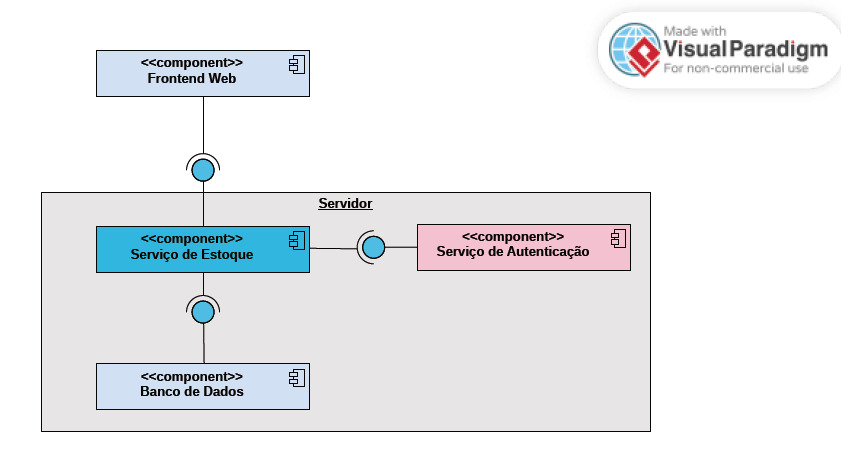
\includegraphics[width=1.0\textwidth]{Figuras/Componentes.png}


\subsubsection{Diagrama de Implantação}


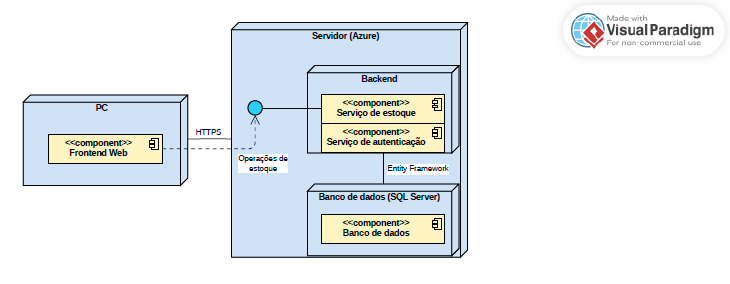
\includegraphics[width=1.0\textwidth]{Figuras/Implantação.png}



\section{Tecnologias}

Esta seção apresenta as principais tecnologias utilizadas no desenvolvimento do sistema, organizadas em categorias como front-end, back-end, banco de dados e infraestrutura. A escolha de cada tecnologia considerou fatores como desempenho, escalabilidade, familiaridade da equipe e compatibilidade com os requisitos do projeto.

\subsection{Front-end}

\begin{itemize}

   \item \textbf{Razor}: Engine de templates do ASP.NET utilizada para gerar as views da aplicação. Permite a criação de páginas HTML dinâmicas por meio da integração entre C\# e marcação HTML, facilitando a renderização de conteúdo no lado do servidor.

   \item \textbf{HTML, CSS e JavaScript}: Tecnologias fundamentais para a construção da camada de apresentação do sistema. O HTML estrutura o conteúdo das páginas, o CSS define o estilo visual e o JavaScript adiciona interatividade ao front-end.

   \item \textbf{Bootstrap}: Framework front-end baseado em HTML, CSS e JS que oferece componentes prontos e responsivos, facilitando a criação de interfaces modernas, padronizadas e adaptáveis a diferentes dispositivos.

   \item \textbf{jQuery}: Biblioteca JavaScript que simplifica a manipulação do DOM, o tratamento de eventos e requisições AJAX. Foi utilizada para agilizar o desenvolvimento de funcionalidades interativas no front-end da aplicação.

\end{itemize}


\subsection{Back-end}

\begin{itemize}

  \item \textbf{C\# com ASP.NET MVC}: Linguagem e framework utilizados na construção do back-end da aplicação, seguindo o padrão arquitetural Model-View-Controller (MVC), que organiza o código de forma modular, separando lógica de negócios, visualização e controle.

  \item \textbf{Entity Framework com LINQ}: Conjunto de tecnologias para acesso a dados em .NET. O Entity Framework permite o mapeamento objeto-relacional (ORM), e o LINQ facilita a realização de consultas ao banco de dados de forma legível e integrada ao C\#.

  \item \textbf{ASP.NET Identity}: Sistema de autenticação e controle de acesso da Microsoft utilizado para gerenciar usuários, perfis e permissões de forma segura e integrada ao projeto. \cite{AspNet2025}.

  \item \textbf{JJMaster Data}: Ferramenta de administração e modelagem de dados que permite a criação dinâmica de formulários e telas de cadastro com base nas entidades do sistema, otimizando o desenvolvimento da interface administrativa.

\end{itemize}

\subsection{Banco de Dados}

\begin{itemize}
    \item \textbf{Microsoft SQL Server}: O Microsoft SQL Server é um sistema de gerenciamento de banco de dados relacional (RDBMS) robusto e amplamente utilizado no mercado, responsável pelo armazenamento seguro das informações da aplicação \cite{SqlServer2025}.


\end{itemize}

\subsection{Infraestrutura}

\begin{itemize}
    \item \textbf{Microsoft Azure}: Plataforma de computação em nuvem utilizada para hospedar a aplicação e seus serviços relacionados. A utilização do Azure proporciona escalabilidade, segurança e alta disponibilidade \cite{Azure2025}.
\end{itemize}



\section{Testes de Manutenção}

\subsection{Plano de Testes}

\subsection{Análise Estatística}

\subsection{Testes Funcionais}

\subsection{Testes Não Funcionais}


\section{Segurança, Privacidade, Legislação}

Este tópico é dedicado a explicar sobre as questões de segurança e legislação relevantes para o nosso projeto.


\subsection{Critérios de Segurança e Privacidade}

O sistema de gerenciamento de estoque foi projetado com critérios de segurança e privacidade para garantir a integridade das informações e proteger os dados dos usuários. As principais medidas adotadas no projeto incluem:

\begin{itemize}
    \item \textbf{Autenticação e Autorização:} O acesso ao sistema é controlado por meio de autenticação de usuários, utilizando o \textit{ASP.NET Identity}. Cada usuário precisa estar autenticado para acessar funcionalidades sensíveis, como cadastro de produtos, movimentação de estoque ou relatórios.

    \item \textbf{Criptografia de Senhas:} As senhas dos usuários são armazenadas de forma criptografada (hash) no banco de dados, conforme práticas recomendadas pelo \textit{Entity Framework}.

    \item \textbf{Boas Práticas de Privacidade:} Os dados pessoais dos usuários, como nome e e-mail, são utilizados apenas para fins de autenticação e gerenciamento interno, e não são compartilhados com terceiros.
\end{itemize}

\subsection{Legislação}

A  Lei Geral de Proteção de Dados (LGPD - Lei nº 13.709/2018) garante transparencia diante ao uso de dados pessoais garantindo que os dados coletados sejam utilizados exclusivamente para fins de autenticação, autorização e controle de acesso ao sistema. Sendo assim, o sistema segue as diretrizes da LGPD, adotando medidas técnicas e administrativas adequadas para proteger os dados pessoais contra acessos não autorizados, perda ou vazamento. 

Além da LGPD, o sistema também considera princípios estabelecidos no Marco Civil da Internet (Lei nº 12.965/2014), que estabelece garantias, direitos e deveres para o uso da internet no Brasil.




\section{Modelo de Banco de Dados}

O modelo de banco de dados é responsável por organizar e estruturar as informações utilizadas no sistema, garantindo integridade, consistência e facilidade no acesso aos dados. Nesta seção, são apresentados o Modelo Entidade-Relacionamento (MER), o Diagrama Entidade-Relacionamento (DER) e o Dicionário de Dados. O MER e o DER representam graficamente as entidades, atributos e relacionamentos do sistema, enquanto o dicionário de dados descreve detalhadamente cada campo presente no banco, incluindo tipo, tamanho e função. O modelo foi projetado para gerenciar de forma eficiente o controle de estoque, permitindo registrar entradas, saídas, usuários, produtos, fornecedores e categorias.

\subsection{MER}

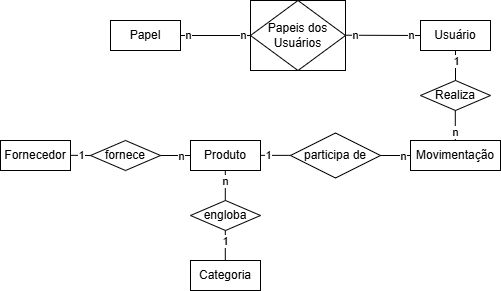
\includegraphics[width=1.0\textwidth]{Figuras/MERestoque.png}


\subsection{DER}

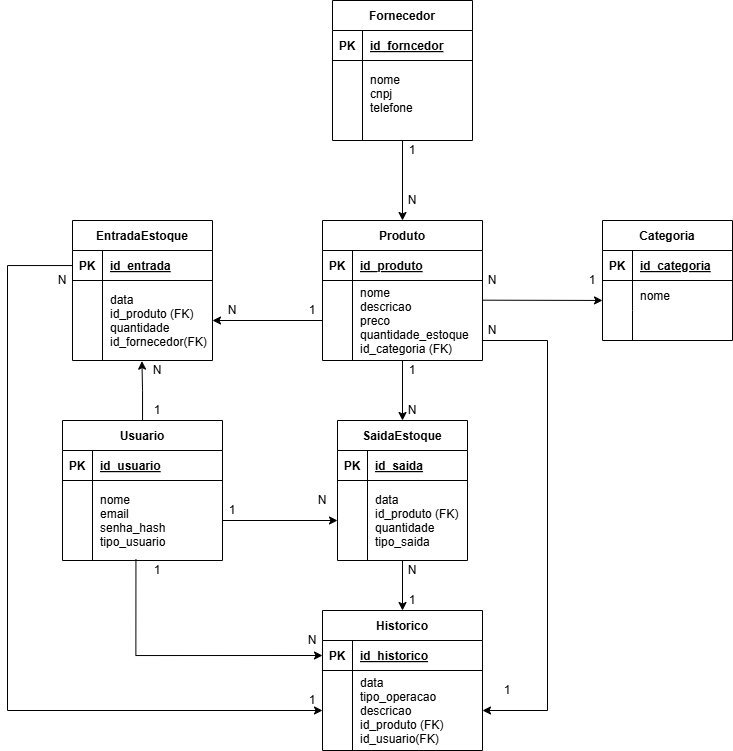
\includegraphics[width=1.0\textwidth]{Figuras/DERestoque.png}



\subsection{Dicionário de Dados}

\section{Cronograma}

Cronograma de Atividades – Primeiro Semestre

O desenvolvimento do sistema de gerenciamento de estoque será realizado ao longo de dois semestres letivos, estando o presente cronograma correspondente às atividades planejadas para o primeiro semestre. Neste período inicial, o foco principal está na fundamentação e planejamento do projeto, bem como na construção da prova de conceito e definição do escopo mínimo viável.

No início do semestre, tem-se a fase de desenvolvimento do tema (Entrega do marco dia 08/04/2025), que contempla a escolha do assunto central do projeto. Nessa etapa, são realizadas as tarefas de definição de um parceiro institucional e levantamento preliminar das necessidades de negócio. Em seguida, inicia-se a análise de requisitos, composta pela elaboração de um formulário de coleta de dados, condução de entrevistas com o parceiro escolhido e o levantamento detalhado dos requisitos funcionais e não funcionais do sistema. Complementarmente, realiza-se um estudo de viabilidade, que envolve entrevistas com os stakeholders e a identificação das necessidades estratégicas para garantir a utilidade e aplicabilidade do sistema proposto.

Posteriormente, desenvolve-se a fase de desenho da aplicação (Entrega do marco dia 29/04/2025), com foco na estruturação técnica da solução. Inicialmente, é feito o projeto do banco de dados, com a criação do Modelo Entidade-Relacionamento (MER) e do Diagrama Entidade-Relacionamento (DER). Na sequência, utiliza-se a linguagem UML para a construção dos diagramas de componentes e de implantação, com o objetivo de representar a arquitetura lógica e física do sistema. Ainda nessa fase, realiza-se a modelagem dos processos de negócio, com a descrição dos fluxos atuais (AS IS) e a proposição dos fluxos futuros (TO BE), identificando melhorias e ajustes esperados com a adoção do novo sistema.

A seguir, passa-se à etapa de prova de conceito (Entrega do marco dia 20/05/2025), na qual se realiza a escolha das tecnologias mais adequadas ao projeto, por meio de uma análise criteriosa das alternativas disponíveis. Também são desenvolvidos os protótipos iniciais, incluindo os scripts de criação do banco de dados, os protótipos de interface de usuário (telas) e o início da implementação do back-end do sistema, a fim de validar os conceitos propostos.

Por fim, inicia-se a fase da criação do MVP (Produto Mínimo Viável) (Entrega do marco dia 17/06/2025). Essa etapa inclui a definição clara do problema a ser resolvido, situando o projeto em seu contexto geral, descrevendo o impacto do problema e delimitando suas causas. Após isso, definem-se as prioridades do sistema, com base em critérios objetivos e identificação das funcionalidades prioritárias. Com essas definições, delimita-se o escopo da aplicação, com a explicitação dos limites do MVP, restrições técnicas e restrições de negócio. Por fim, identificam-se as funcionalidades mínimas essenciais, o fluxo principal do usuário no sistema e as integrações necessárias com outros sistemas ou serviços.

Paralelamente, é elaborada a fase de análise e documentação, cujo objetivo é consolidar os dados obtidos até aqui. (Entrega do marco dia 18/07/2025). Esta seção inclui a elaboração da introdução do trabalho, apresentando os objetivos, o problema e a solução proposta. Também se realiza uma breve revisão da literatura, com a recuperação do histórico e contexto do tema. No que se refere à gestão do projeto, descreve-se a organização da equipe e a metodologia adotada. A seção de desenvolvimento do projeto apresenta o escopo definido, seguido pela análise de viabilidade financeira, com a estimativa de custos envolvidos. Por fim, as considerações finais trazem as principais dificuldades encontradas, decisões tomadas e funcionalidades ou ideias descartadas durante o processo.

\subsection{Análise da duração do projeto}

\chapter{Viabilidade Financeira}

\subsection{Custos}
O custo do projeto aqui.

\subsection{Receitas}

\subsection{Cenários}



\chapter{Considerações Finais}
teste

\section{Dificuldades, escolhas}



% ---

\lipsum[24]

% ----------------------------------------------------------
% Finaliza a parte no bookmark do PDF
% para que se inicie o bookmark na raiz
% e adiciona espaço de parte no Sumário
% ----------------------------------------------------------
\phantompart




% ----------------------------------------------------------
% ELEMENTOS PÓS-TEXTUAIS
% ----------------------------------------------------------
\postextual
% ----------------------------------------------------------

% ----------------------------------------------------------
% Referências bibliográficas
% ----------------------------------------------------------
\bibliographystyle{abntex2-alf}
\bibliography{referencias}

% ----------------------------------------------------------
% Glossário
% ----------------------------------------------------------
%
% Consulte o manual da classe abntex2 para orientações sobre o glossário.
%
%\glossary

% ----------------------------------------------------------
% Apêndices
% ----------------------------------------------------------

% ---
% Inicia os apêndices
% ---
\begin{apendicesenv}

% Imprime uma página indicando o início dos apêndices
\partapendices

% ----------------------------------------------------------
\chapter{apendice exemplo}
% ----------------------------------------------------------

\lipsum[50]

% ----------------------------------------------------------
\chapter{Nullam elementum urna vel imperdiet sodales elit ipsum pharetra ligula
ac pretium ante justo a nulla curabitur tristique arcu eu metus}
% ----------------------------------------------------------
\lipsum[55-57]

\end{apendicesenv}
% ---


% ----------------------------------------------------------
% Anexos
% ----------------------------------------------------------

% ---
% Inicia os anexos
% ---
\begin{anexosenv}

% Imprime uma página indicando o início dos anexos
\partanexos

% ---
\chapter{exemplo 2}
% ---
\lipsum[30]

% ---
\chapter{Cras non urna sed feugiat cum sociis natoque penatibus et magnis dis
parturient montes nascetur ridiculus mus}
% ---

\lipsum[31]

% ---
\chapter{exemplo 3}
% ---

\lipsum[32]

\end{anexosenv}

%---------------------------------------------------------------------
% INDICE REMISSIVO
%---------------------------------------------------------------------
\phantompart
\printindex
%---------------------------------------------------------------------

\end{document}
